\section{Arquitetura de sistema}
A figura~\ref{fig:46} expõe a arquitetura do sistema que indica as principais componentes. Entre estas, é possível visualizar a aplicação \textit{frontend}, que realiza pedidos a uma aplicação \textit{backend} e espera respostas. O \textit{backend} é composto por uma \textit{\textit{\acrshort{api}} rest} que recebe e responde aos pedidos e por uma base de dados a qual recebe \textit{queries} e devolve dados para a \textit{\textit{\acrshort{api}} rest}. Encontra-se no documento de anexos, no anexo 20, uma versão mais detalhada da Figura~\ref*{fig:46}.

\begin{figure}[htb]
  \centering
  
  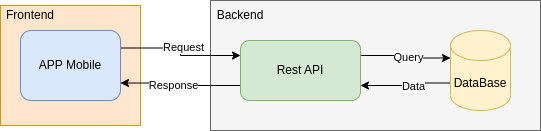
\includegraphics[width=0.8\textwidth]{images/Arquiteturas/arquitetura_de_solucao.png}
  \caption{Arquitetura do sistema}
  \label{fig:46}
\end{figure}

\newpage

\subsection{Arquitetura de funcional}
A especificação da implementação da \textit{\textit{\acrshort{api}} rest} foi realizada através de uma arquitetura de \textit{backend}(Figura~\ref{fig:47}). Aqui, é possível visualizar que sempre que a \textit{\acrshort{api}} recebe um pedido, este é redirecionado primeiramente para o \textit{router}. O \textit{router} tem como função identificar a rota referente ao pedido e deslocar para os respetivos \textit{middlewares}. 

Os \textit{middlewares} têm como objetivo realizar todas as ações necessárias antes de proceder à execução do código de rota. Os \textit{middlewares} existentes são o \textit{SessionTokenValidator}, valida a sessão do utilizador a realizar o pedido, de forma similar, o \textit{middleware RefreshTokenValidator}, valida a sessão principal do utilizador e por fim, o \textit{middleware} \textit{RoleValidator}, valida se o utilizador que efetua o pedido tem cargos suficientes para tal. Na eventualidade de não existir nenhum impedimento, o pedido é direcionado para o \textit{controller}.

O \textit{controller} extrai os dados do pedido, verifica se os dados obrigatórios existem e cumprem as regras de negócio e encaminha o pedido para o serviço. O serviço, em caso de necessidade, irá proceder à interação com a base de dados, esta realiza diversas ações como, obter, atualizar, apagar e inserir dados. Por fim, após todo o código de serviço ser executado, a resposta é formulada e devolvida para o utilizador.

Encontra-se no documento de anexos, no anexo 21, uma versão mais detalhada da Figura~\ref*{fig:47}.

\begin{figure}[htb]
  \centering
  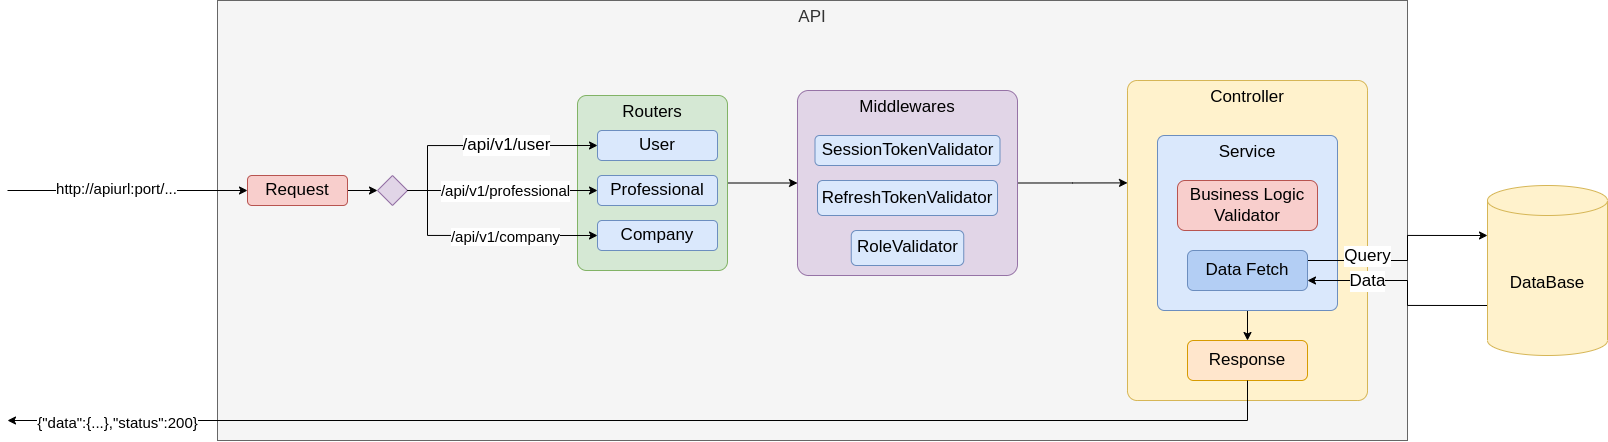
\includegraphics[width=0.9\textwidth]{images/Arquiteturas/arquitetura_funcional.png}
  \caption{Arquitetura funcional}
  \label{fig:47}
\end{figure}

\newpage

\subsection{Arquitetura de serviços}
A arquitetura de serviços contém todos os serviços que deverão ser implementados no \textit{frontend}, com a identificação dos atores que poderão realizar estes pedidos. Esta foi desenvolvida após uma análise de todos os dados necessários para suporte do \textit{frontend}.

\begin{figure}[htb]
  \centering
  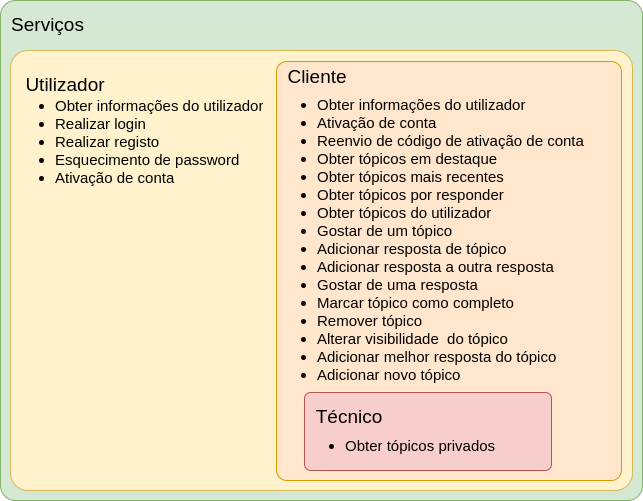
\includegraphics[width=0.8\textwidth]{images/Arquiteturas/arquitetura_de_componentes_final.png}
  \caption{Arquitetura de componentes}
  \label{fig:48}
\end{figure}

\newpage

\subsection{Tabela de endpoints}
Com o propósito de evitar colisões de \textit{endpoints} durante a implementação, foi desenvolvida uma tabela de \textit{endpoints}. Esta possui dados semelhantes à arquitetura de componentes (Figura~\ref*{fig:48}), mas para cada serviço é indicada a rota e o método a utilizar.

Encontra-se no documento de anexos, no anexo 25, uma versão mais detalhada da Figura~\ref*{docs_swagger}.

% \usepackage{color}
% \usepackage{tabularray}
\definecolor{Concrete}{rgb}{0.952,0.952,0.952}
\begin{longtblr}
[
caption={Tabela de endpoints},
label={tab:19},
]{
  row{1} = {Concrete,c},
  hlines,
  vlines,
}
Serviço                                    & Ator       & Rota                                                             & Método \\
{Obter informações \\do utilizador}        & Cliente    & baseurl/client/:uid                                              & GET    \\
Realizar login                             & Utilizador & baseurl/login                                                    & POST   \\
Realizar registo                           & Utilizador & baseurl/register                                                 & POST   \\
{Esquecimento de \\password}               & Utilizador & baseurl/forgot-password                                          & GET    \\
Ativação de conta                          & Cliente & baseurl/client/:uid/activate                                     & POST   \\
{Reenvio de código \\de ativação de conta} & Cliente & baseurl/client/:uid/new-code                                     & GET    \\
{Obter tópicos em \\destaque}              & Cliente    & baseurl/client/topics/featured                                   & GET    \\
{Obter tópicos mais \\recentes}            & Cliente    & baseurl/client/topics/latest                                     & GET    \\
{Obter tópicos por \\responder}            & Cliente    & baseurl/client/topics/to-answer                                  & GET    \\
{Obter tópicos do \\utilizador}            & Cliente    & baseurl/client/topics                                            & GET    \\
{Obter tópicos \\privados}                 & Técnico    & baseurl/professional/topics/private                              & GET    \\
{Gostar de um \\tópico}                    & Cliente    & baseurl/client/topics/:topicId/like                              & PUT    \\
{Adicionar resposta \\a tópico}            & Cliente    & baseurl/client/topics/:topicId/answer                            & POST   \\
{Adicionar resposta \\a outra resposta}    & Cliente    & baseurl/client/answers/:answerId/                                & POST   \\
{Gostar de uma \\resposta}                  & Cliente    & baseurl/client/answers/:answerId/like                            & PUT    \\
{Marcar tópico \\como completo}            & Cliente    & baseurl/client/topics/:topicId/completed                         & PUT    \\
Remover Tópico                             & Cliente    & baseurl/client/topics/:topicId/                                  & DELETE \\
{Alterar visibilidade \\do tópico}         & Cliente    & baseurl/client/topics/:topicId/visibility                        & PUT    \\
{Adicionar melhor \\resposta do tópico}    & Cliente    & {baseurl/client/topics/:topicId/answers/\\:answerId/best-answer} & PUT    \\
Adicionar novo tópico                      & Cliente    & baseurl/client/topics/                                           & POST   
\end{longtblr}

\begin{figure}[htb]
  \centering
  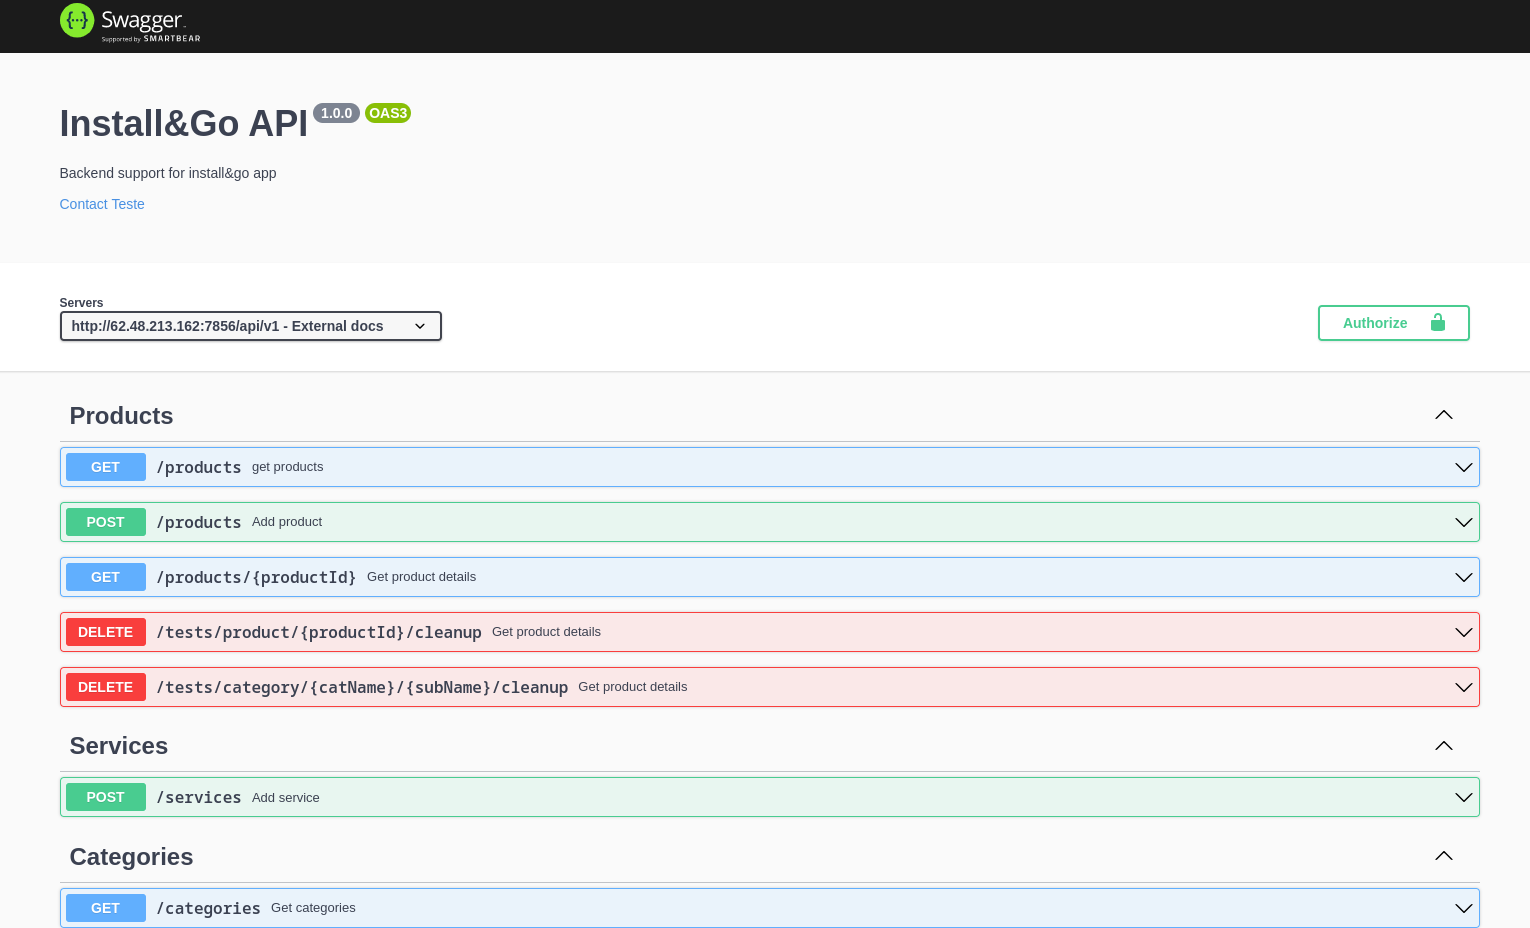
\includegraphics[width=\textwidth]{images/implementacao/api/swagger_intro.png}
  \caption{Listagem de serviços documentados}
  \label{docs_swagger}
\end{figure}

\newpage
